\documentclass{beamer}

\usepackage{fontspec,xunicode,xltxtra}

\usepackage{tikz}%TiKZ绘图
\usetikzlibrary{arrows,shapes,chains}
\usetikzlibrary{graphs, positioning, quotes, shapes.geometric}
\usepackage{array}
\usepackage{amsmath}%数学公式相关
\usepackage{amssymb}%更多的数学符号
\usepackage{caption}%控制题目/说明文字的样式
\usepackage{graphicx, subfig}%插入图片
\usepackage{float}%强行保留图片位置用

\XeTeXlinebreaklocale "zh"
%\XeTeXlinebreakskip = 0pt plus 1pt minus 0.1pt

%\setmainfont[Mapping=tex-text]{AR PL UMing CN:style=Light}
%\setmainfont[Mapping=tex-text]{AR PL UKai CN:style=Book}
%\setmainfont[Mapping=tex-text]{WenQuanYi Zen Hei:style=Regular}
%\setmainfont[Mapping=tex-text]{WenQuanYi Zen Hei Sharp:style=Regular}
%\setmainfont[Mapping=tex-text]{AR PL KaitiM GB:style=Regular} 
%\setmainfont[Mapping=tex-text]{AR PL SungtiL GB:style=Regular} 
%\setmainfont[Mapping=tex-text]{WenQuanYi Zen Hei Mono:style=Regular} 

%\newfontfamily\hei{WenQuanYi Micro Hei}
%\newfontfamily\whei{WenQuanYi Zen Hei}
\newfontfamily\kai{AR PL UKai CN}
\newfontfamily\song{AR PL UMing CN}
%\newfontfamily\bhei{cwTeXHeiBold}
%\newfontfamily\lishu{SIMLI}
%\setmainfont[Mapping=tex-text]{WenQuanYi Micro Hei}
\setsansfont[Mapping=tex-text]{AR PL UKai CN}
%\setmonofont[Mapping=tex-text]{WenQuanYi Zen Hei Mono}

%\renewcommand{\baselinestretch}{1.25}


\mode<presentation>
{
	\usetheme{Darmstadt}
	
	% \usetheme{Warsaw}
	% or ...
	%  \usetheme{default}
	
	\setbeamercovered{transparent}
	% or whatever (possibly just delete it)
}


\usepackage[english]{babel}
% or whatever

%\usepackage[latin1]{inputenc}
% or whatever

\title[Beamer + xelatex] % (optional, use only with long paper titles)
{\Huge Julia 集的分析和探索}

%\subtitle
%{第一讲: 进入真正的计算机世界} % (optional)

\author[Wu HY] % (optional, use only with lots of authors)
{吴泓鹰}
% - Use the \inst{?} command only if the authors have different
%   affiliation.

\institute[ZJU] % (optional, but mostly needed)
{
	数学与应用数学(强基计划)\\
	3210101890
}
% - Use the \inst command only if there are several affiliations.
% - Keep it simple, no one is interested in your street address.

\date[] % (optional)
{2022年7月4日}

% If you have a file called "university-logo-filename.xxx", where xxx
% is a graphic format that can be processed by latex or pdflatex,
% resp., then you can add a logo as follows:

\logo{
\includegraphics[height=1cm]{../png/zju.jpg}}

\begin{document}
	
\begin{frame}
	\titlepage % Print the title page as the first slide
\end{frame}

\begin{frame}
	\frametitle{目录}
	\tableofcontents
\end{frame}

\begin{frame}{引入:问题背景}
\section{引入:问题背景}
Julia集由法国数学家Gaston Julia发现并命名,其是在复平面上构成分形点的集合。在复动力系统的背景下,Julia集由使得任意小的扰动就会使迭代函数序列发生剧烈变化的值组成,这体现了Julia集行为上的混沌性。关于Julia集有很多有趣和美丽的地方,下面我们将对Julia集进行简单的分析和探索。
\end{frame}

\begin{frame}{分析:生成Julia集/数学原理}
\section{分析:生成Julia集}
\begin{itemize}
\item Julia集一般可以定义为使得复函数$f_c(z)=z^2+c$经过无数次迭代后能够不发散的复数$z$的集合,其中$c\in\mathbb{C}$,我们一般取$|c|<2$。
\item 进一步的,令$f(z)$为有理函数,其定义为$\displaystyle f(z):=\frac{p(z)}{q(z)}$,其中$z\in\mathbb{C}^*,\mathbb{C}^*$为黎曼球面$\mathbb{C}\bigcup\{\infty\}$,$p,q$为没有公因式的多项式。则拓展后的Julia集$J_R$为在经过无数次$f(z)$迭代后不发散的$z$的集合,而真正的Julia集$J$为$J_R$的边界$\partial J_R$。
\end{itemize}
\end{frame}

\begin{frame}{分析:生成Julia集/算法实现(流程图)}
	\begin{figure}[H]
		\tikzstyle{io} = [trapezium, trapezium left angle = 60, trapezium right angle = 120, minimum width = 1cm, text centered, draw = black, fill = white, align=center]
		\centering
		\begin{tikzpicture}[node distance=10pt]
			\node[draw, rounded corners](start){开始};
			\node[draw, below=of start](step 1){设置坐标系长宽$a,b$与$i=0$};
			\node[draw, below=of step 1](step 2){设置每个像素占长宽$d$};
			\node[draw, below=25pt of step 2](step 3){取每个像素的复值$z$};
			\node[draw, io, right=of step 2](input){输入复常数$c$\\与迭代次数$N$};
			\node[draw, diamond, aspect=2, below=of input] (choice 1) {$|z|<2$};
			\node[draw, diamond, aspect=2, below=of choice 1] (choice 2) {$i<N$};
			\node[draw, below=30pt of step 3] (step 4) {$z=f(z),i=i+1$};
			\node[draw, right=of choice 2] (step 5) {对像素赋$i$对应的颜色};
			\node[draw, below=of step 5] (step 6) {设置图片$dpi$};
			\node[draw, io , left=30pt of step 6] (step 7) {输出\texttt{.png}图片};
			\node[draw, rounded corners, below=of step 4] (end) {结束};
			
			\draw[->] (choice 1) --node[above] {否} (choice 1 -|step 5) -> (step 5);
			\graph{
				(start) -> (step 1) -> (step 2) -> (input) -> (choice 1) -> ["是"left](choice 2) ->["是"above](step 4) -> (choice 1);
				(step 2) ->["取遍每个像素"left] (step 3) -> (choice 1);
				(choice 2) ->["否"above](step 5) -> (step 6) -> (step 7) -> (end);
			};
		\end{tikzpicture}
	\end{figure}
\end{frame}

\begin{frame}{探索:不同条件下的Julia集/改变迭代次数$N$}
\section{探索:不同条件下的Julia集}
\begin{figure}[H]
	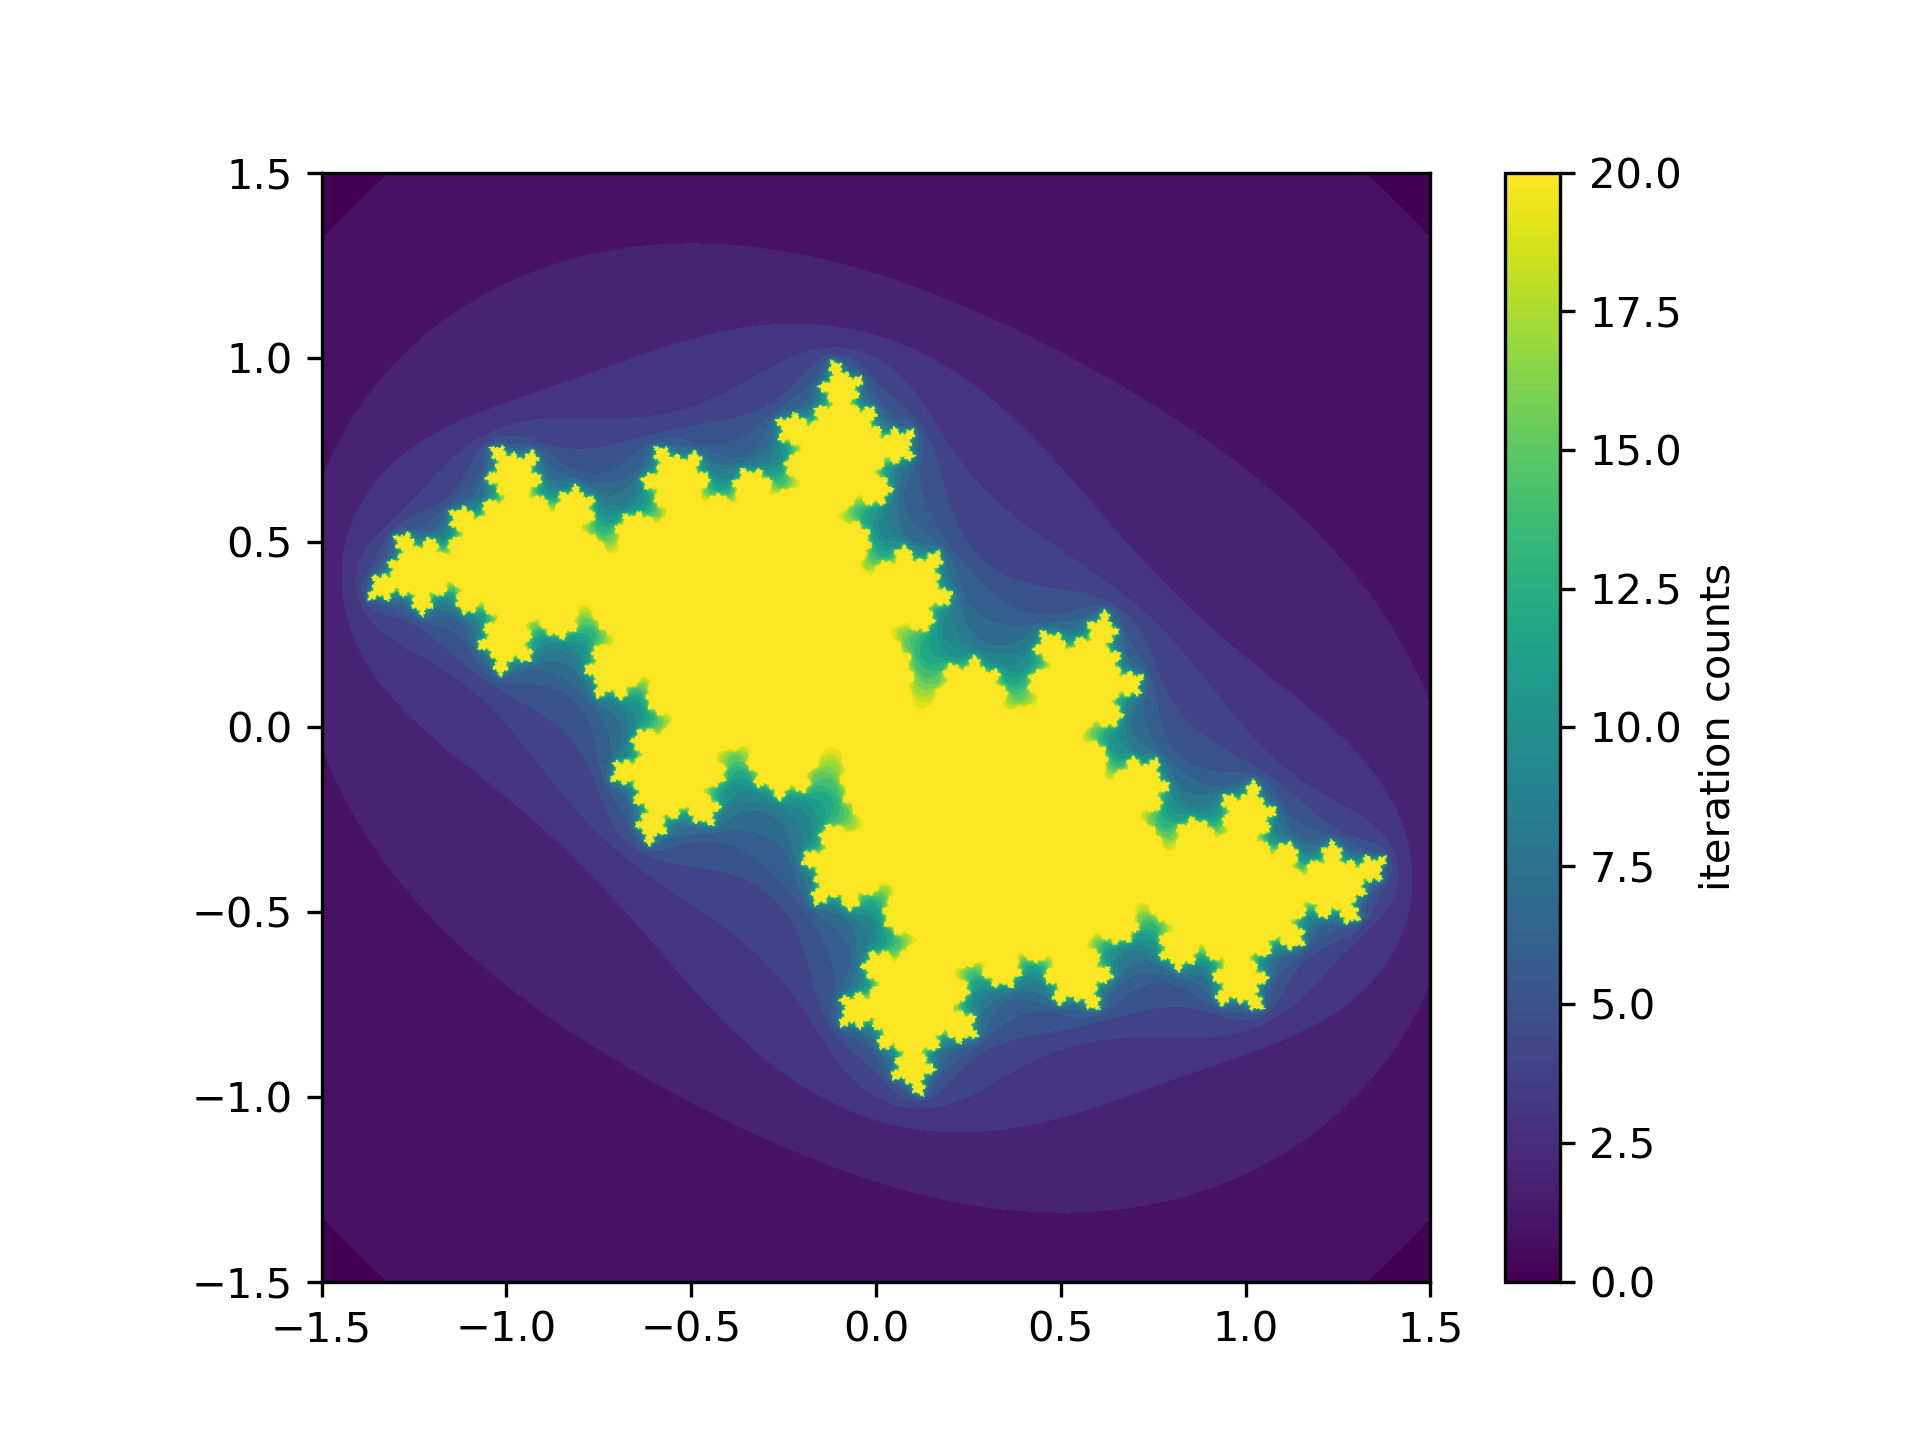
\includegraphics[width=.4\textwidth]{../png/300dpi/julia_cx-0.4cy0.6_N20.png}
	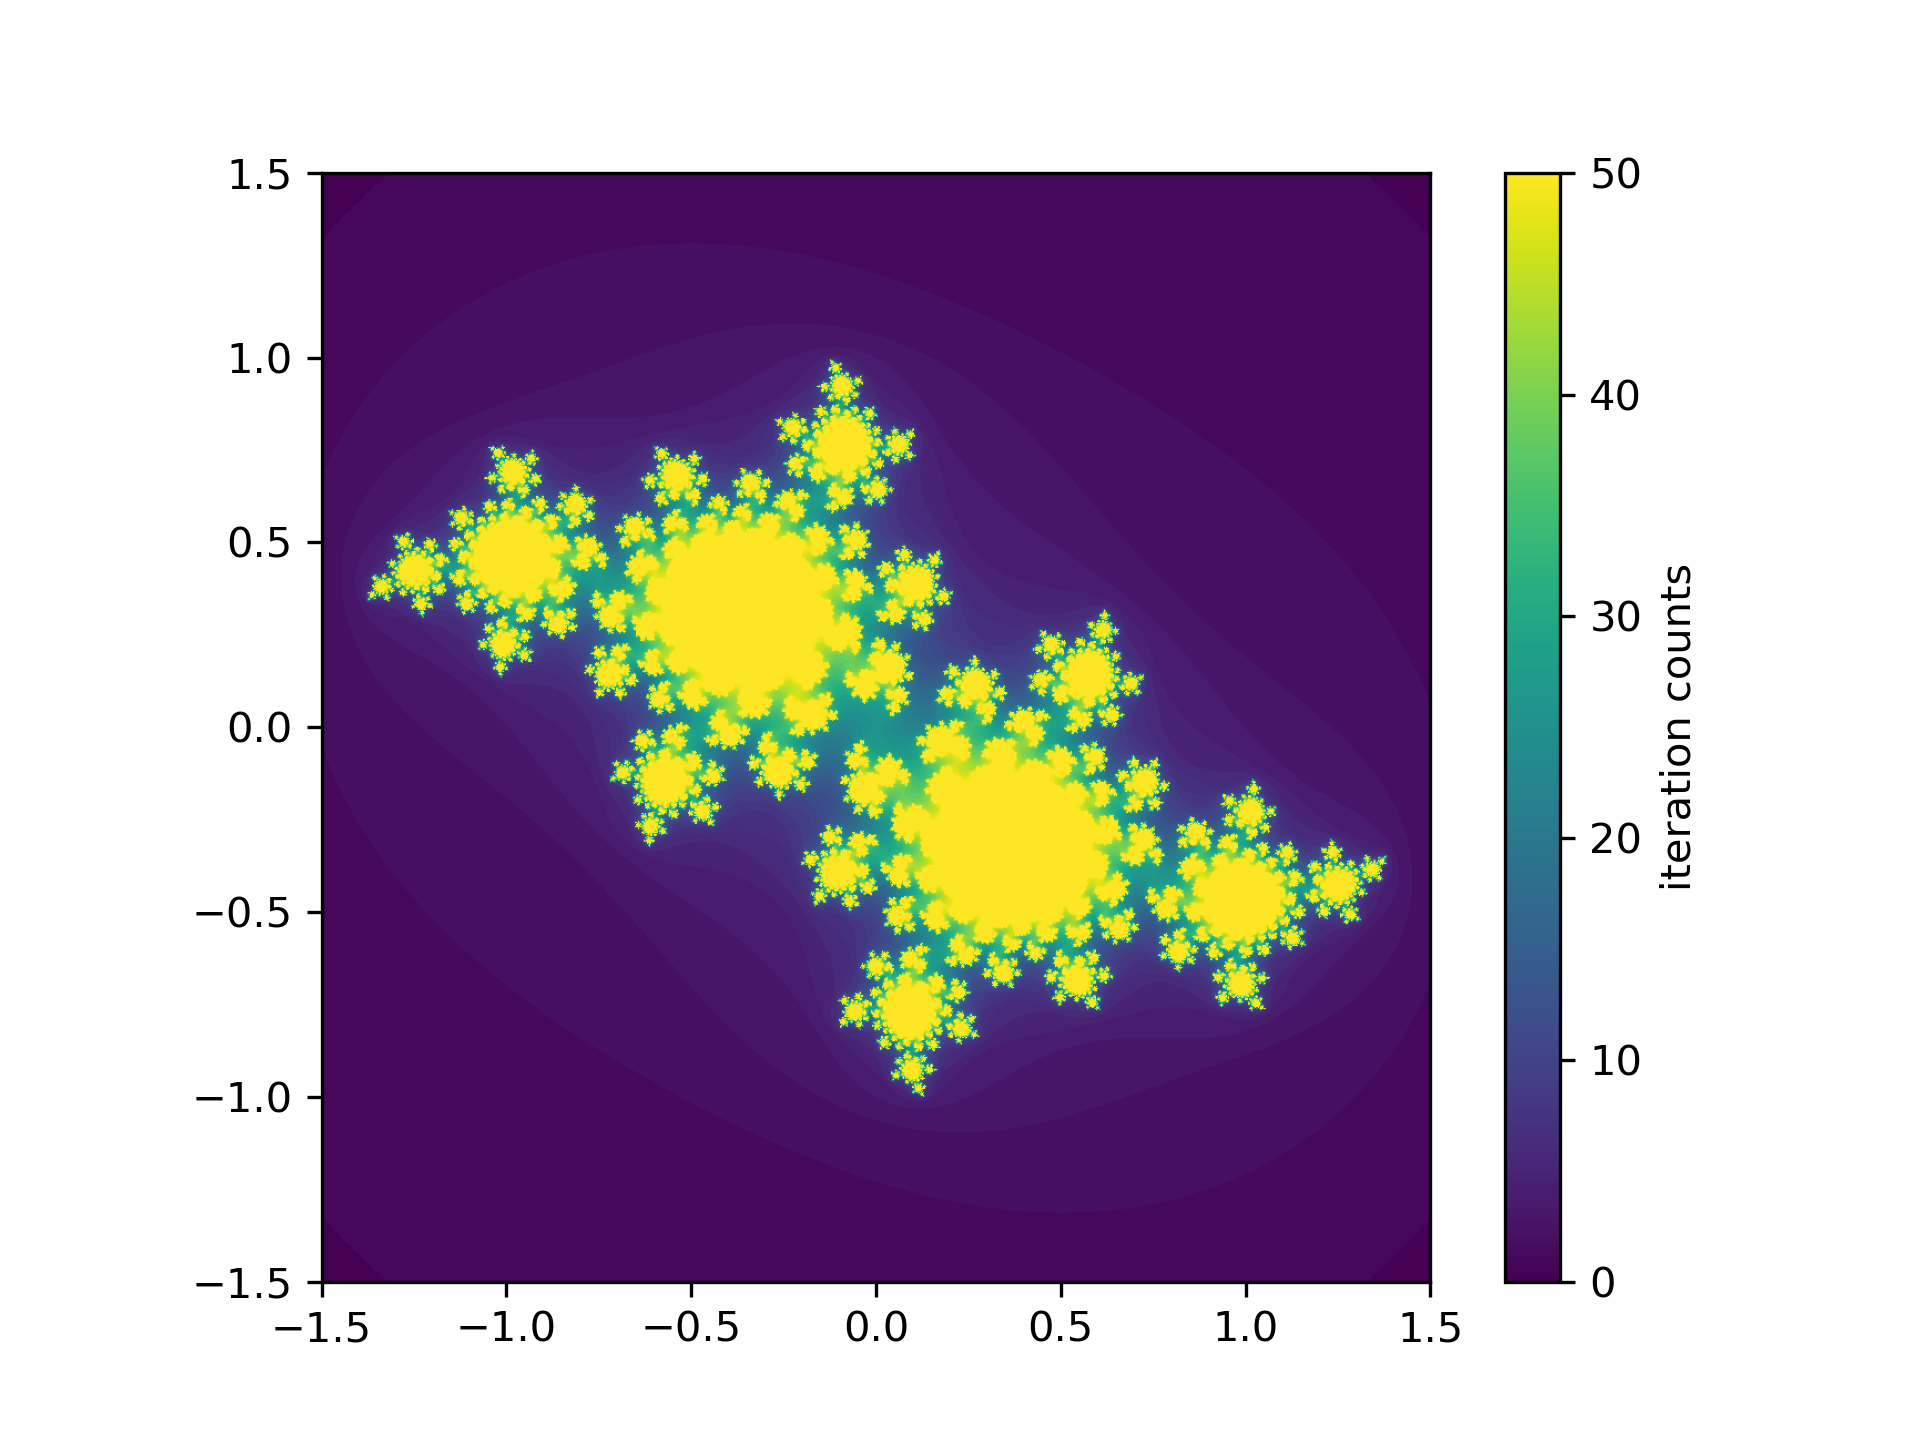
\includegraphics[width=.4\textwidth]{../png/300dpi/julia_cx-0.4cy0.6_N50.png}
	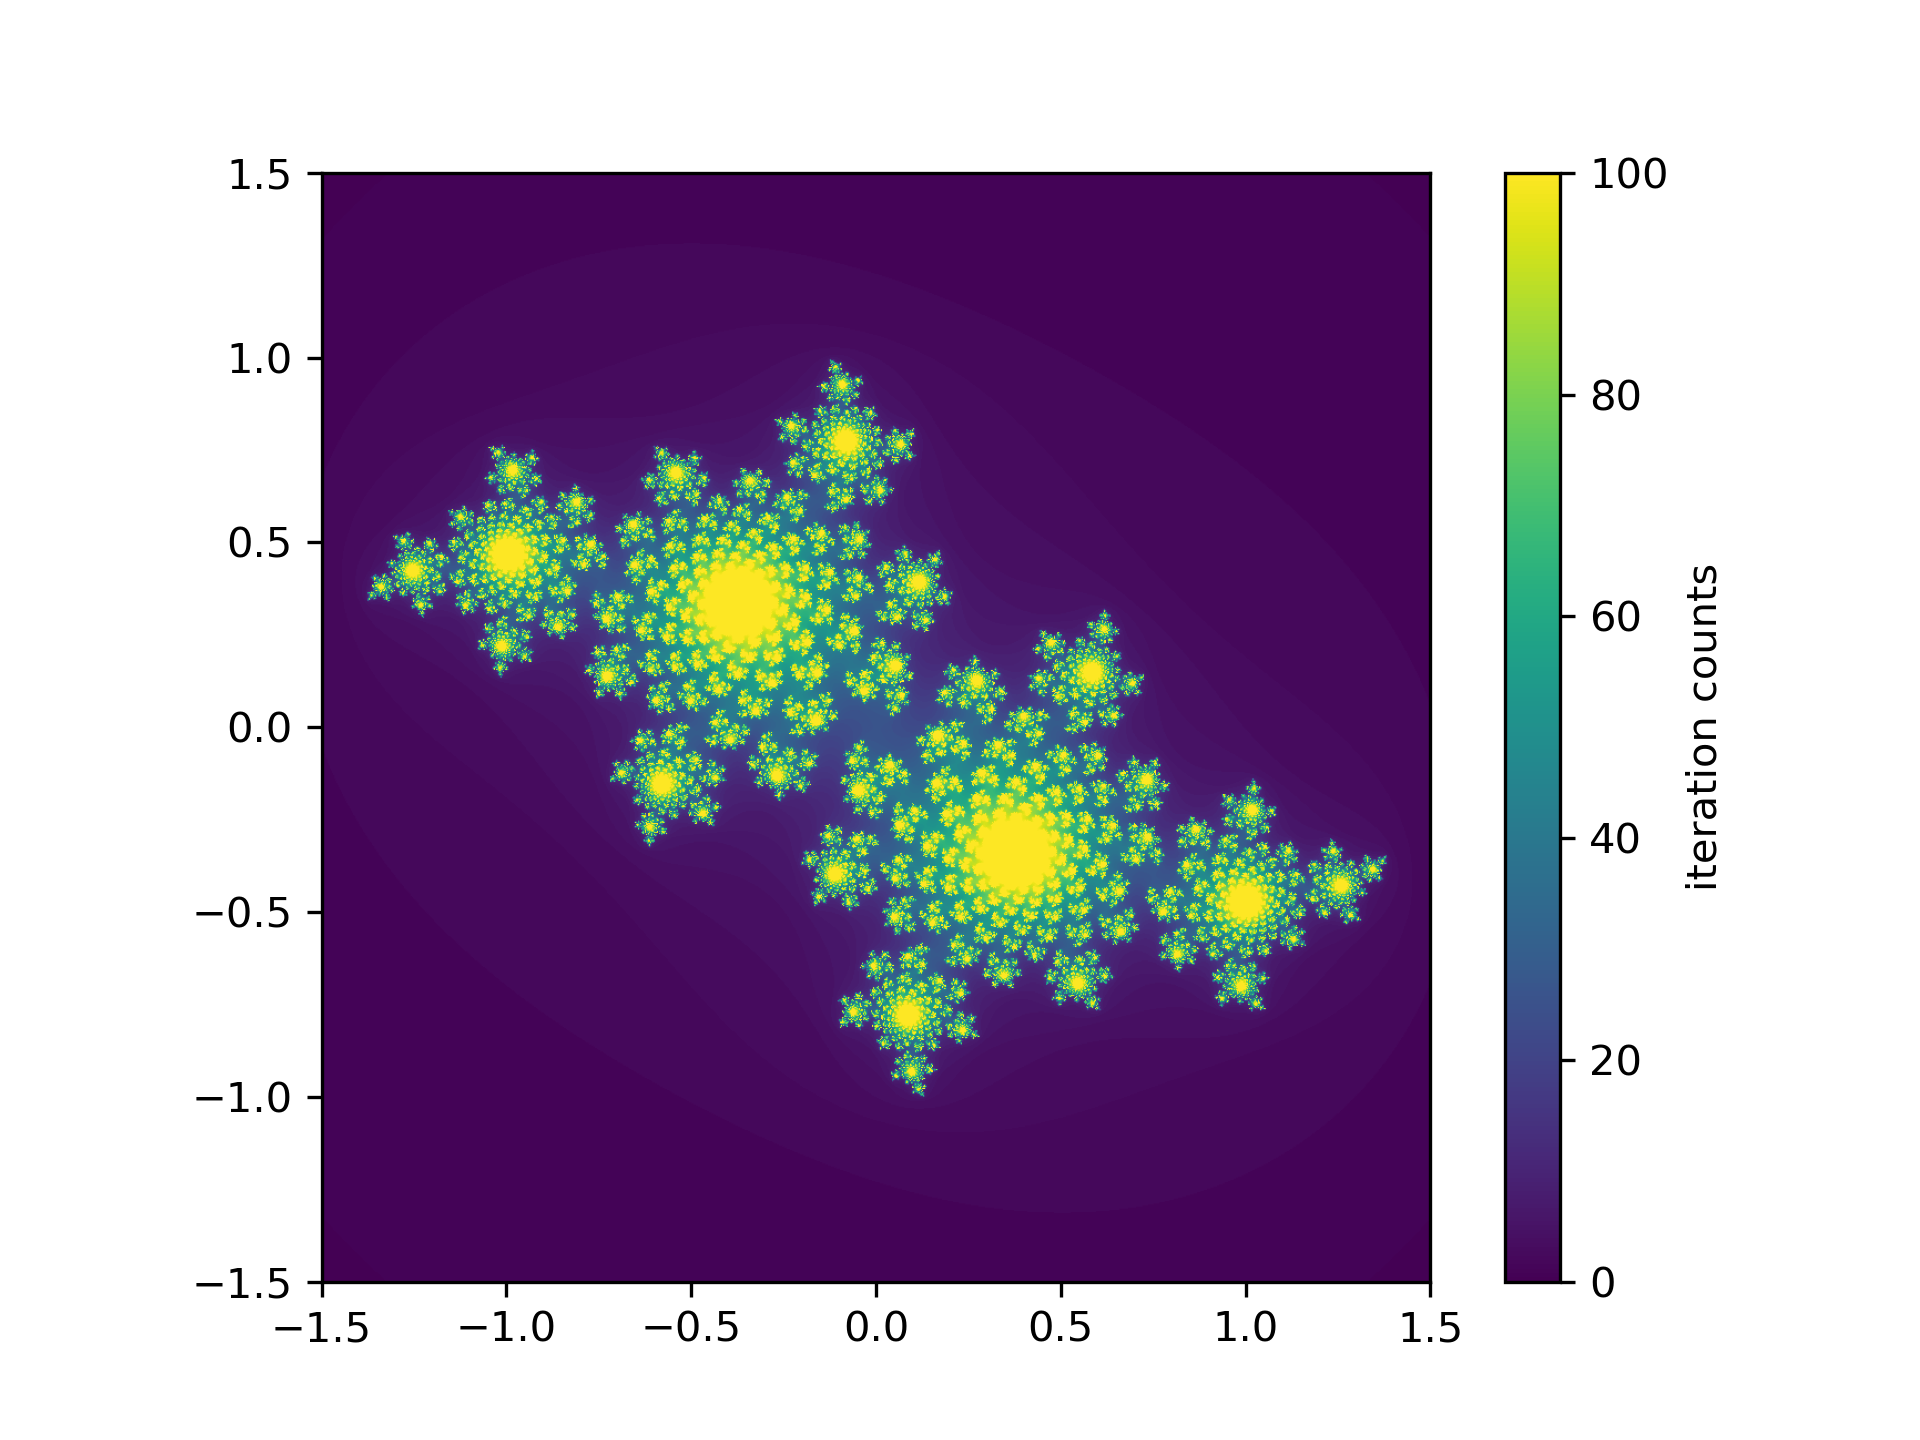
\includegraphics[width=.4\textwidth]{../png/300dpi/julia_cx-0.4cy0.6_N100.png}
	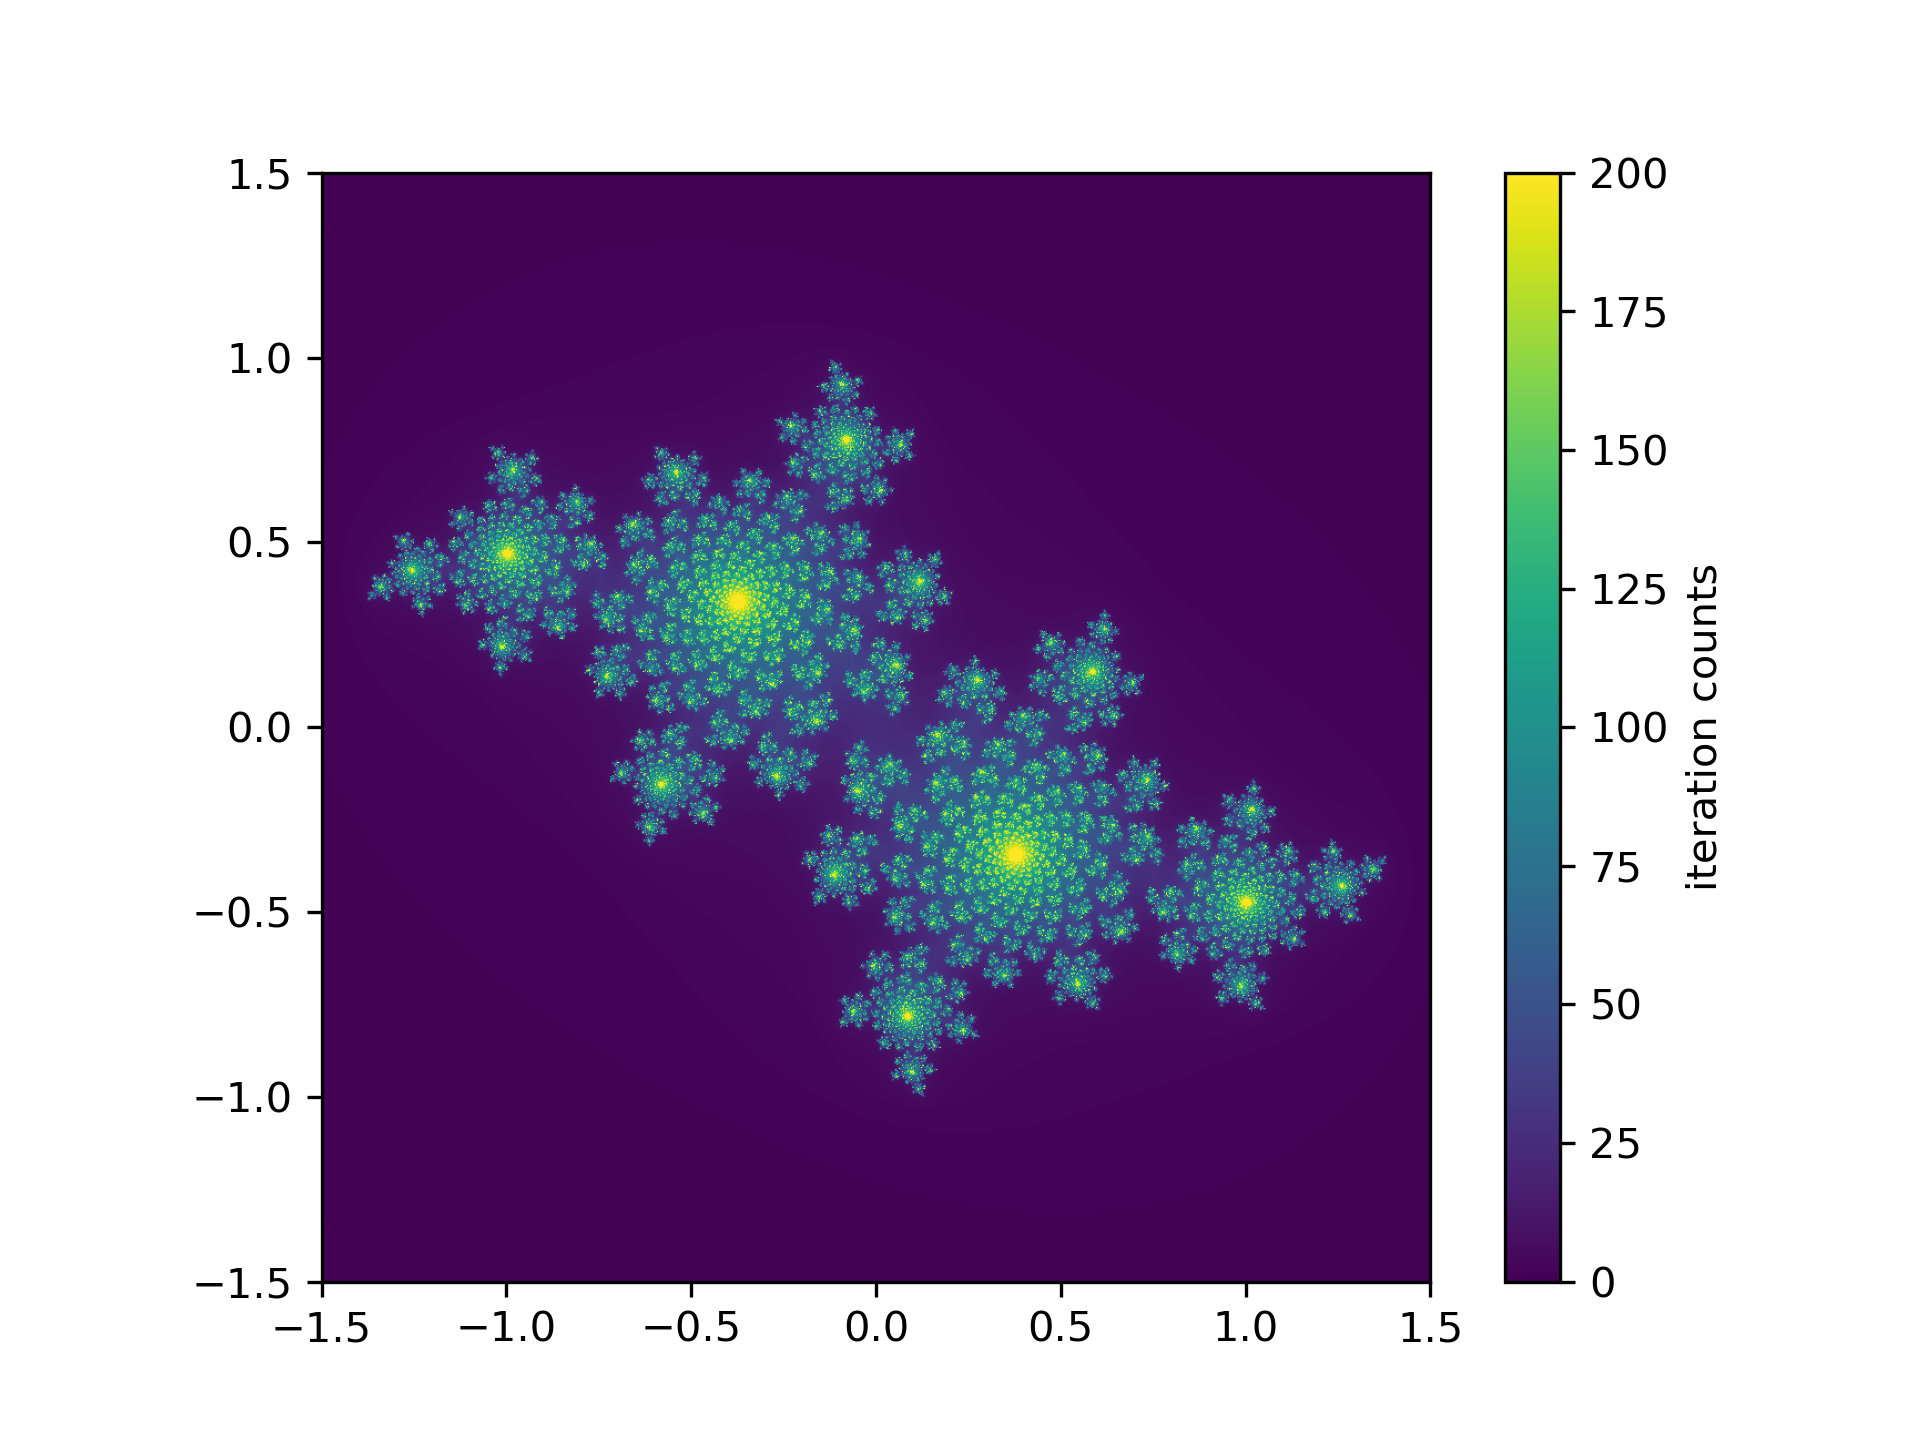
\includegraphics[width=.4\textwidth]{../png/300dpi/julia_cx-0.4cy0.6_N200.png}
	\caption{$c=-0.4+0.6i,N=20,50,100,200$}
\end{figure}
\end{frame}

\begin{frame}{探索:不同条件下的Julia集/改变复常数$c$}
	$c_1=-0.4+0.6i,c_2=-0.8i$,\\$c_3=0.285+0.01i,c_4=-0.8+0.156i$
\begin{figure}[H]
	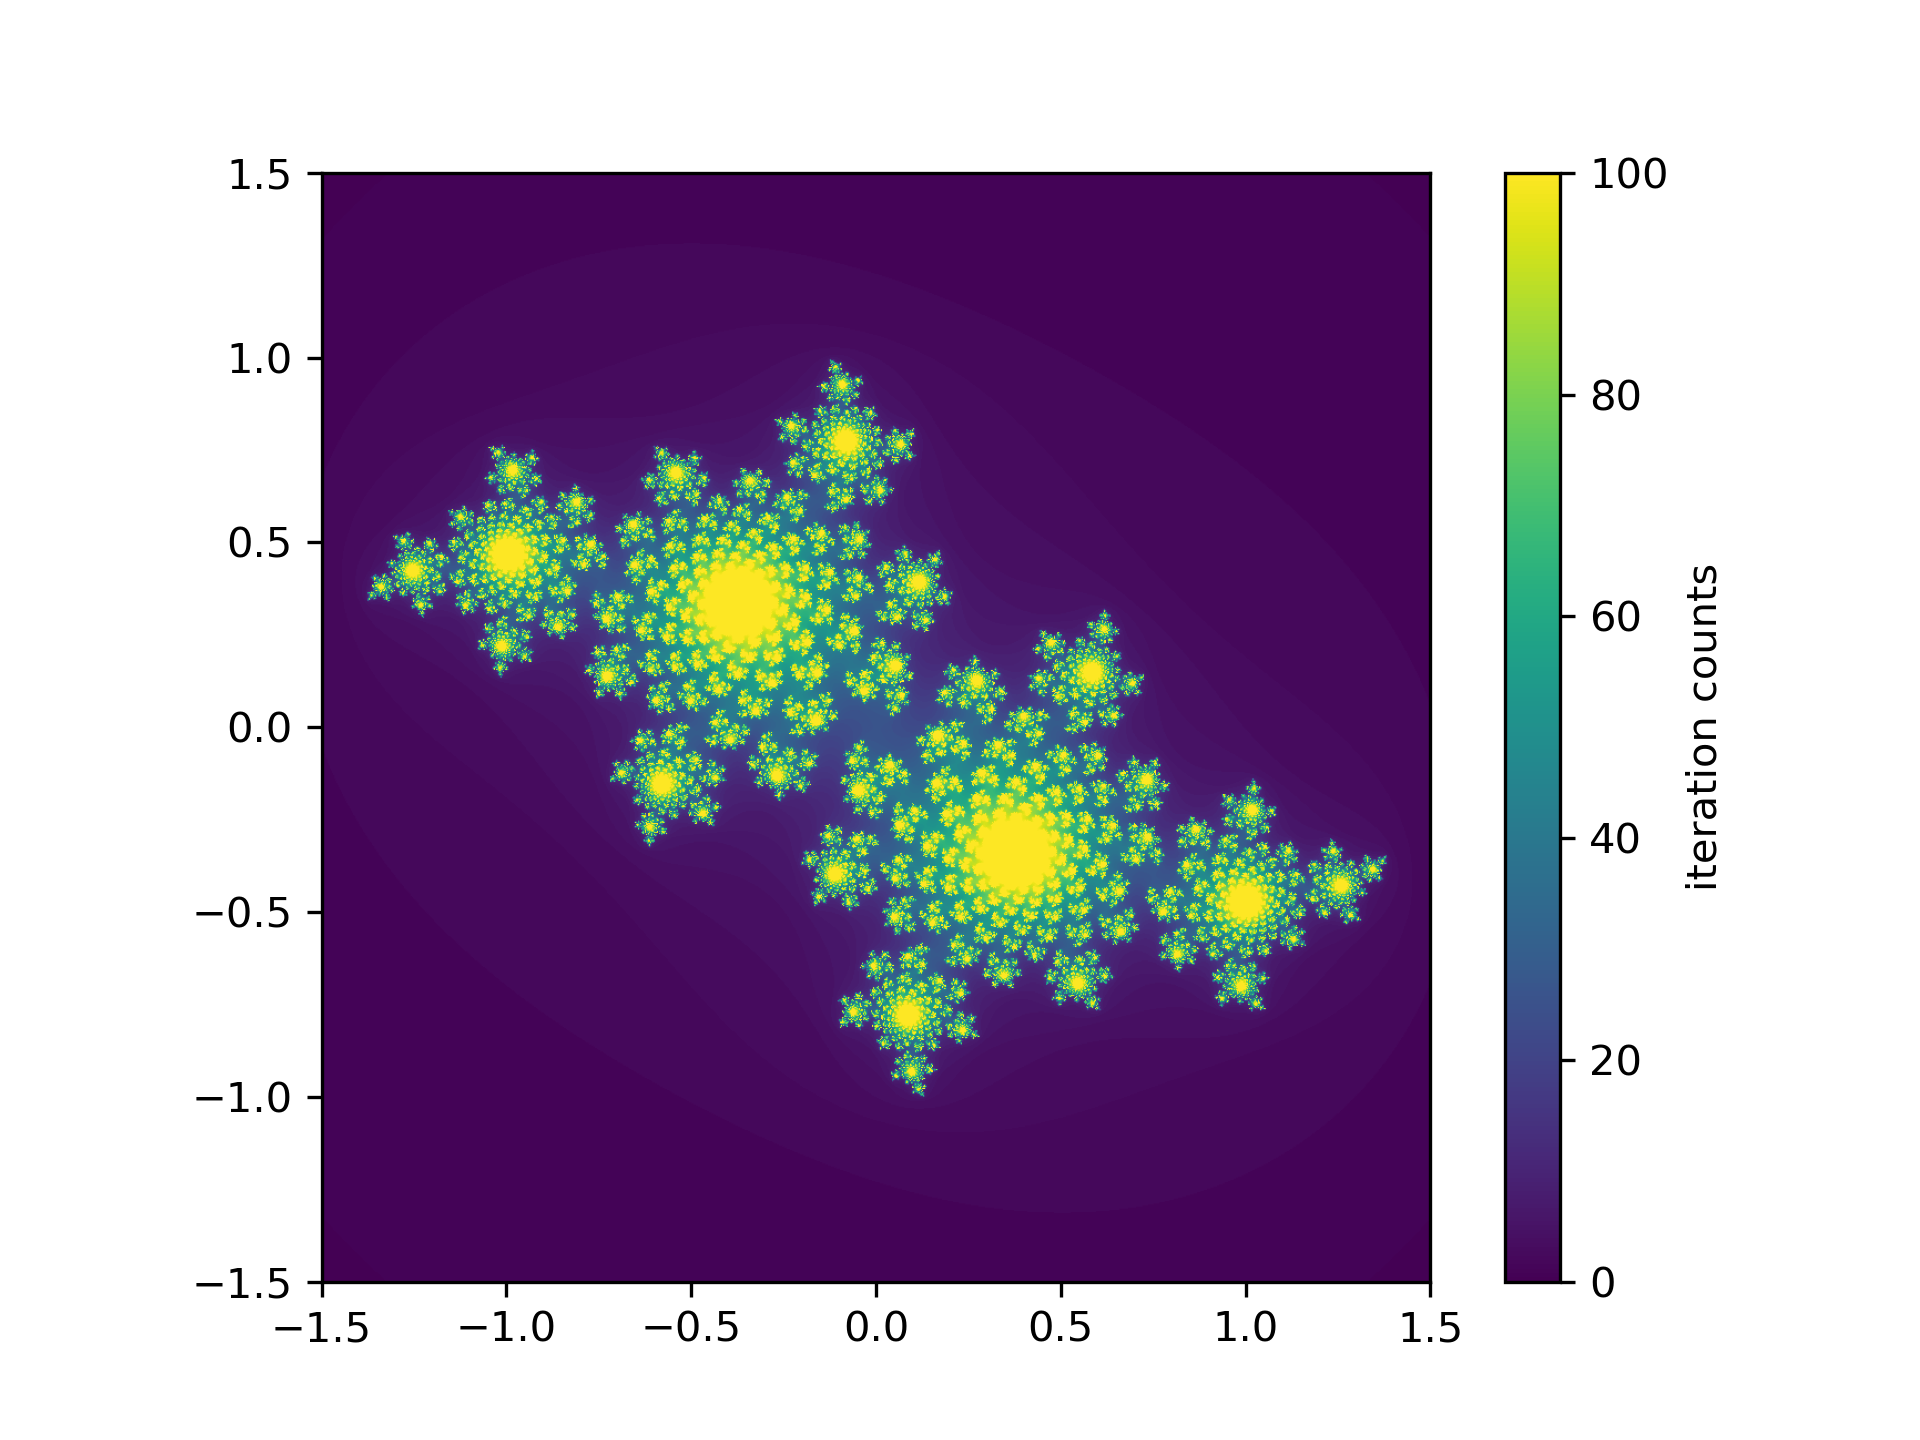
\includegraphics[width=.35\textwidth]{../png/300dpi/julia_cx-0.4cy0.6_N100.png}
	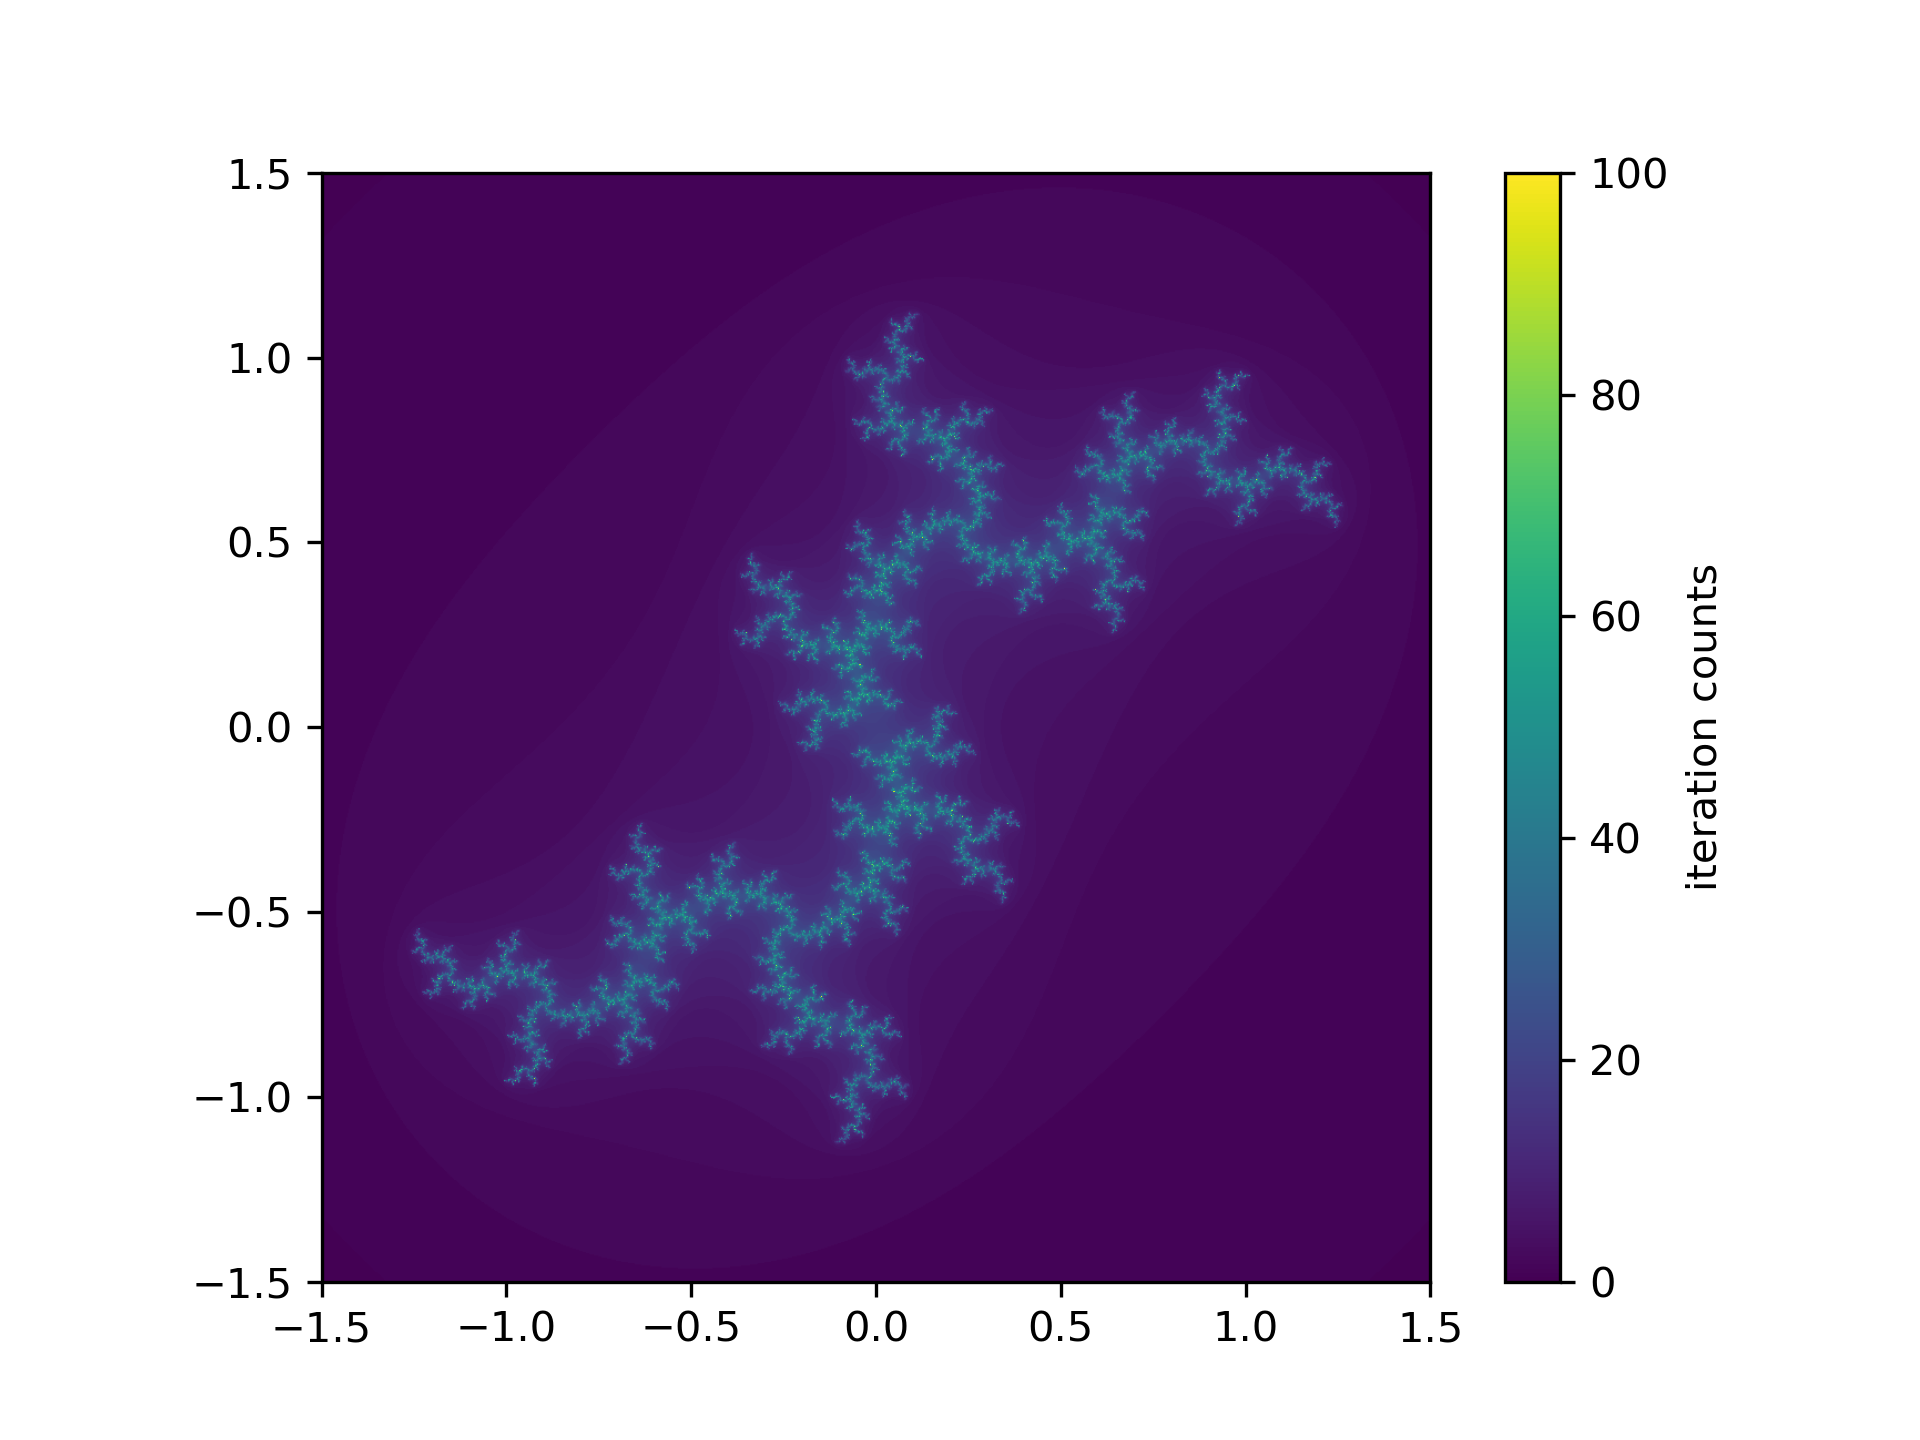
\includegraphics[width=.35\textwidth]{../png/300dpi/julia_cx0cy-0.8_N100.png}
	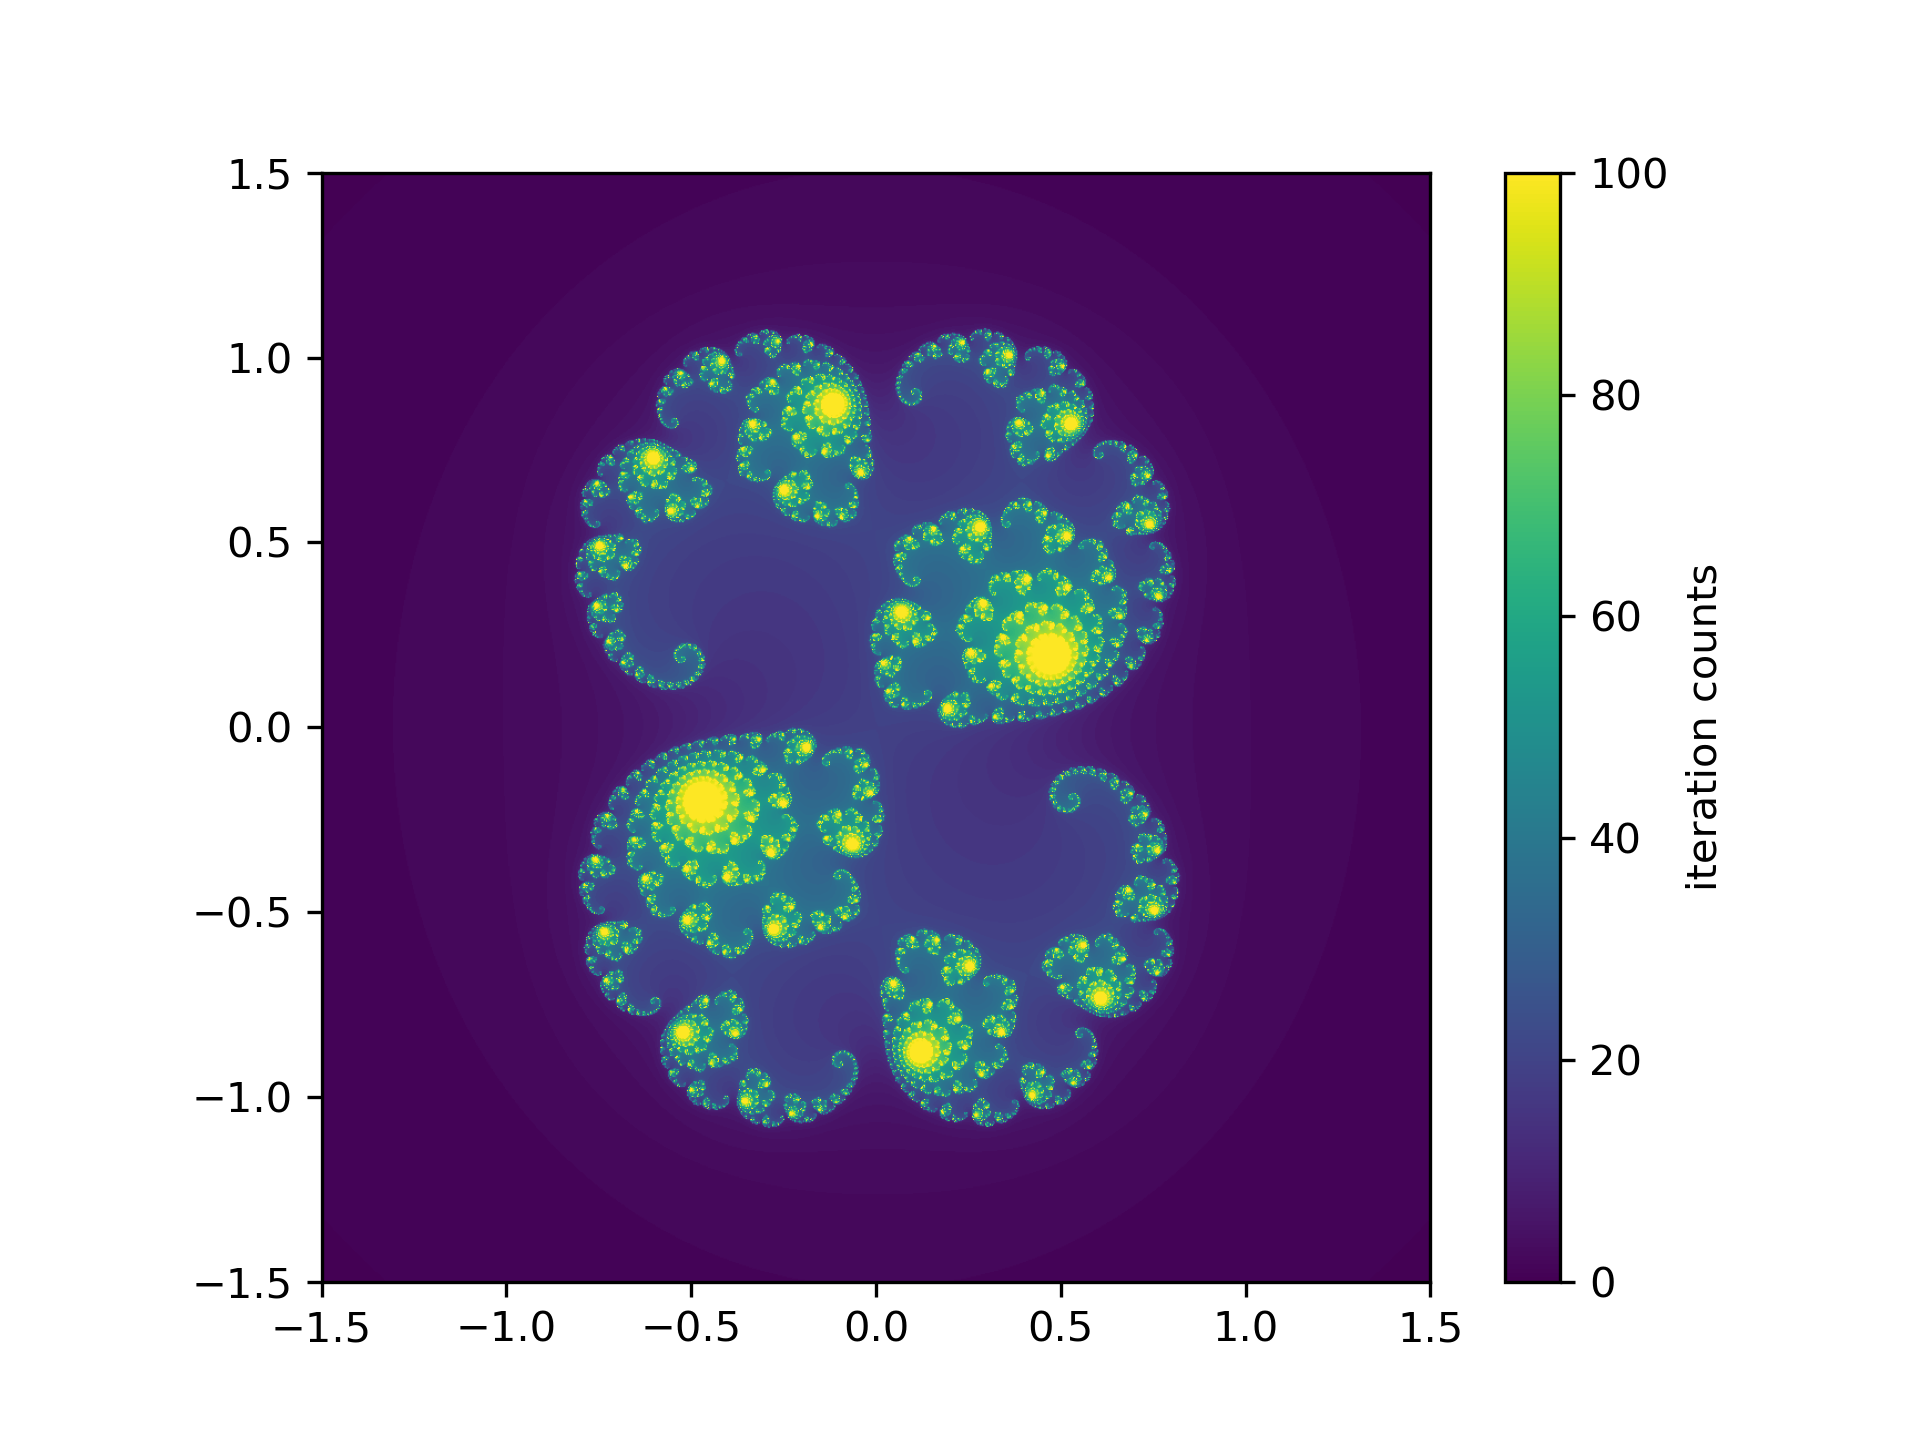
\includegraphics[width=.35\textwidth]{../png/300dpi/julia_cx0.285cy0.01_N100.png}
	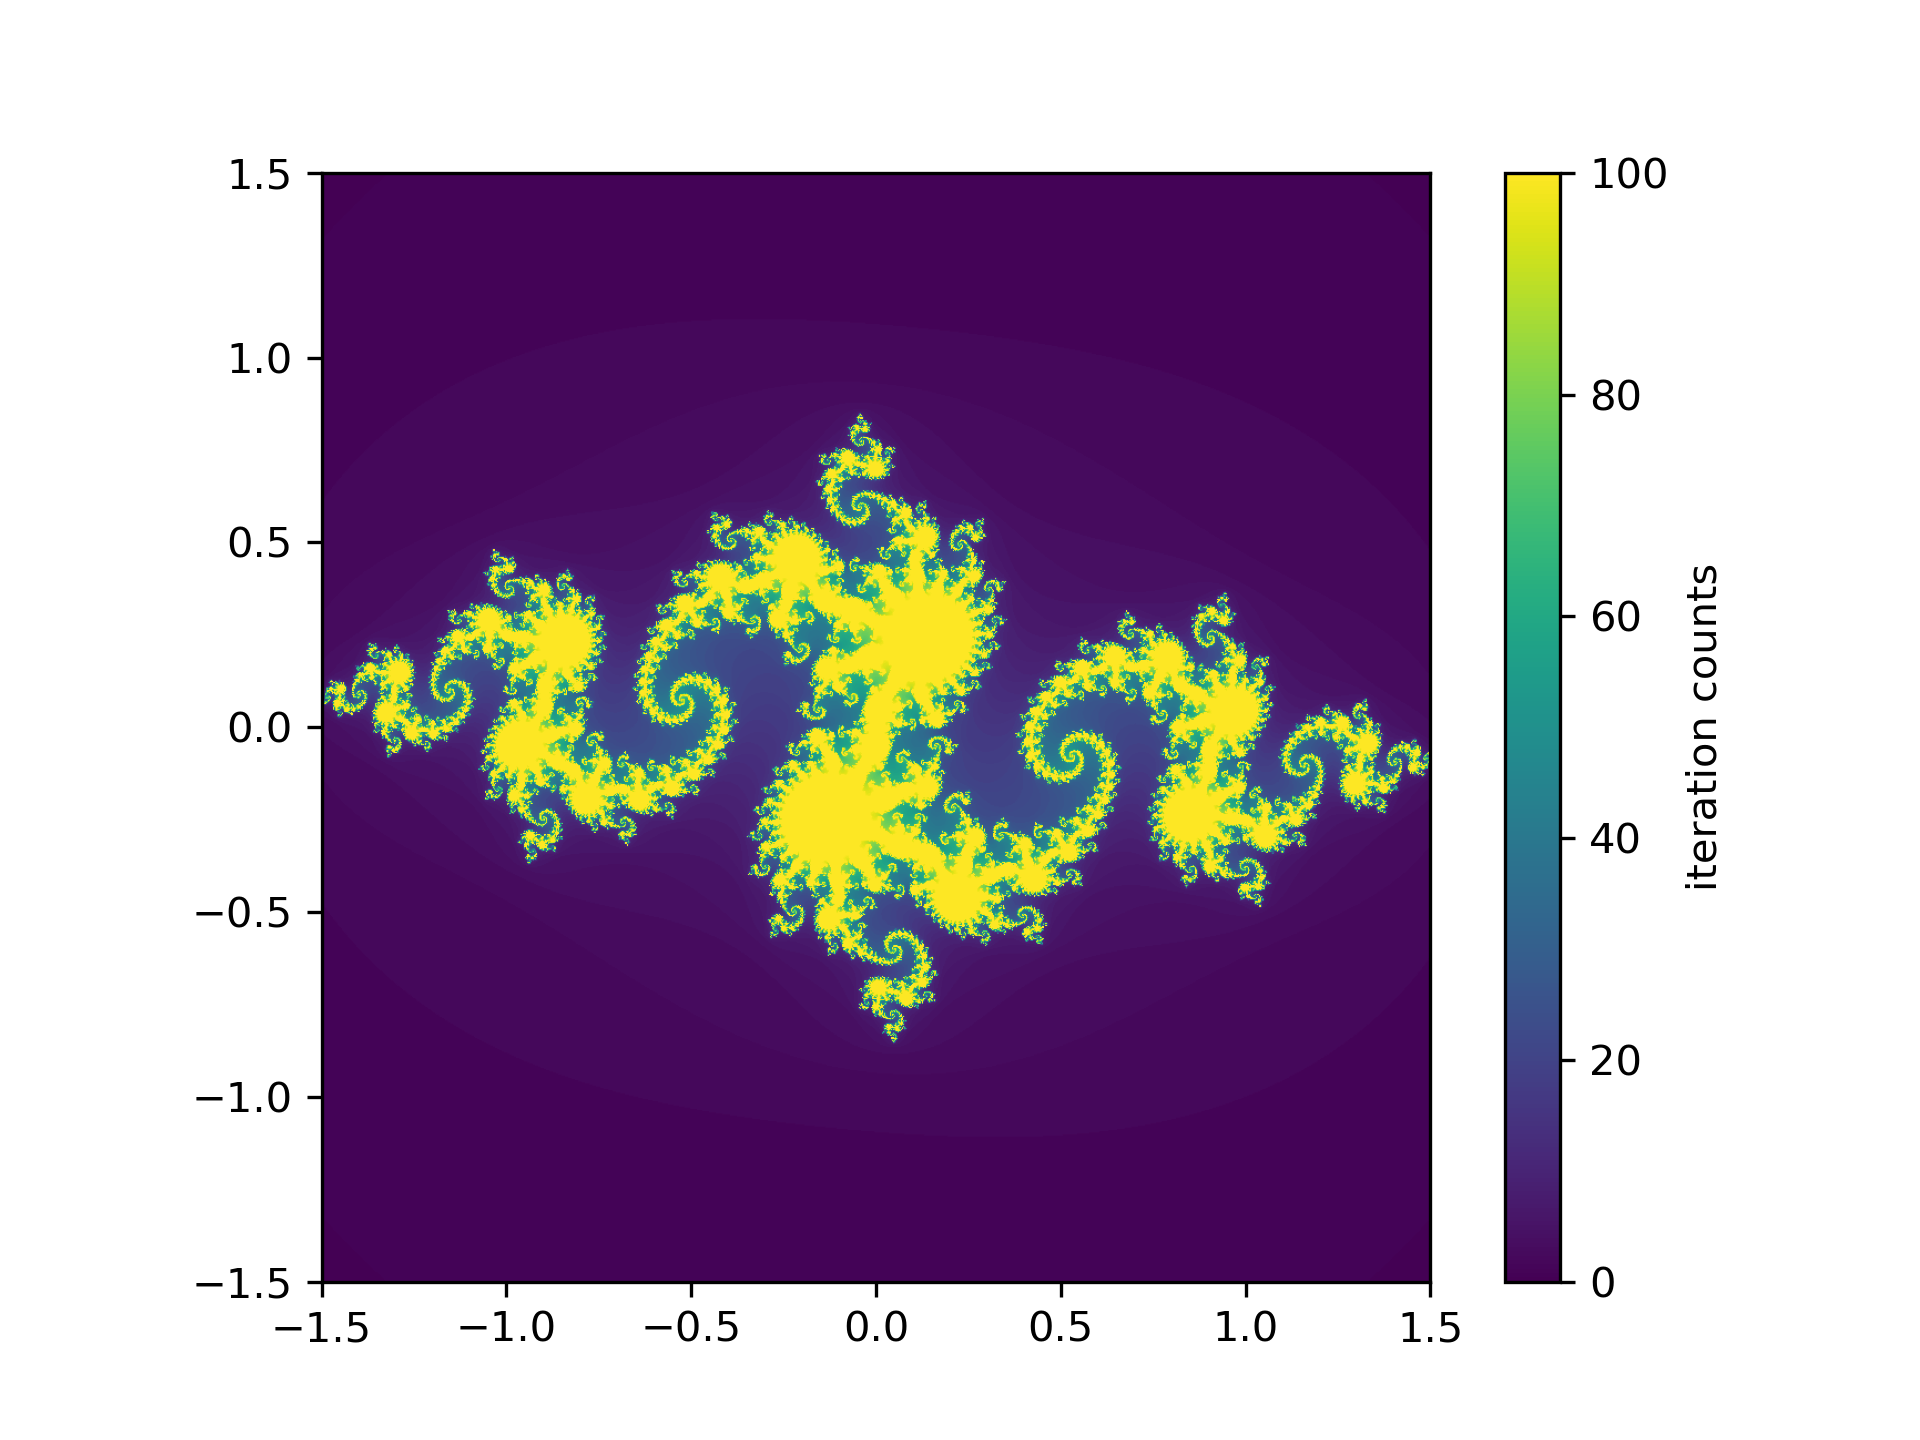
\includegraphics[width=.35\textwidth]{../png/300dpi/julia_cx-0.8cy0.156_N100.png}
	\caption{$N=100,c=c_1,c_2,c_3,c_4$}
\end{figure}

\end{frame}

\begin{frame}{探索:不同条件下的Julia集/改变迭代公式$f(z)$}
	$f_1(z)=z^3-0.071-1.134i$,\\$\displaystyle f_2(z)=\frac{(1-\frac{z^3}{6})}{(z-\frac{z^2}{2})^2}-0.616+0.45i$
\begin{figure}[H]
	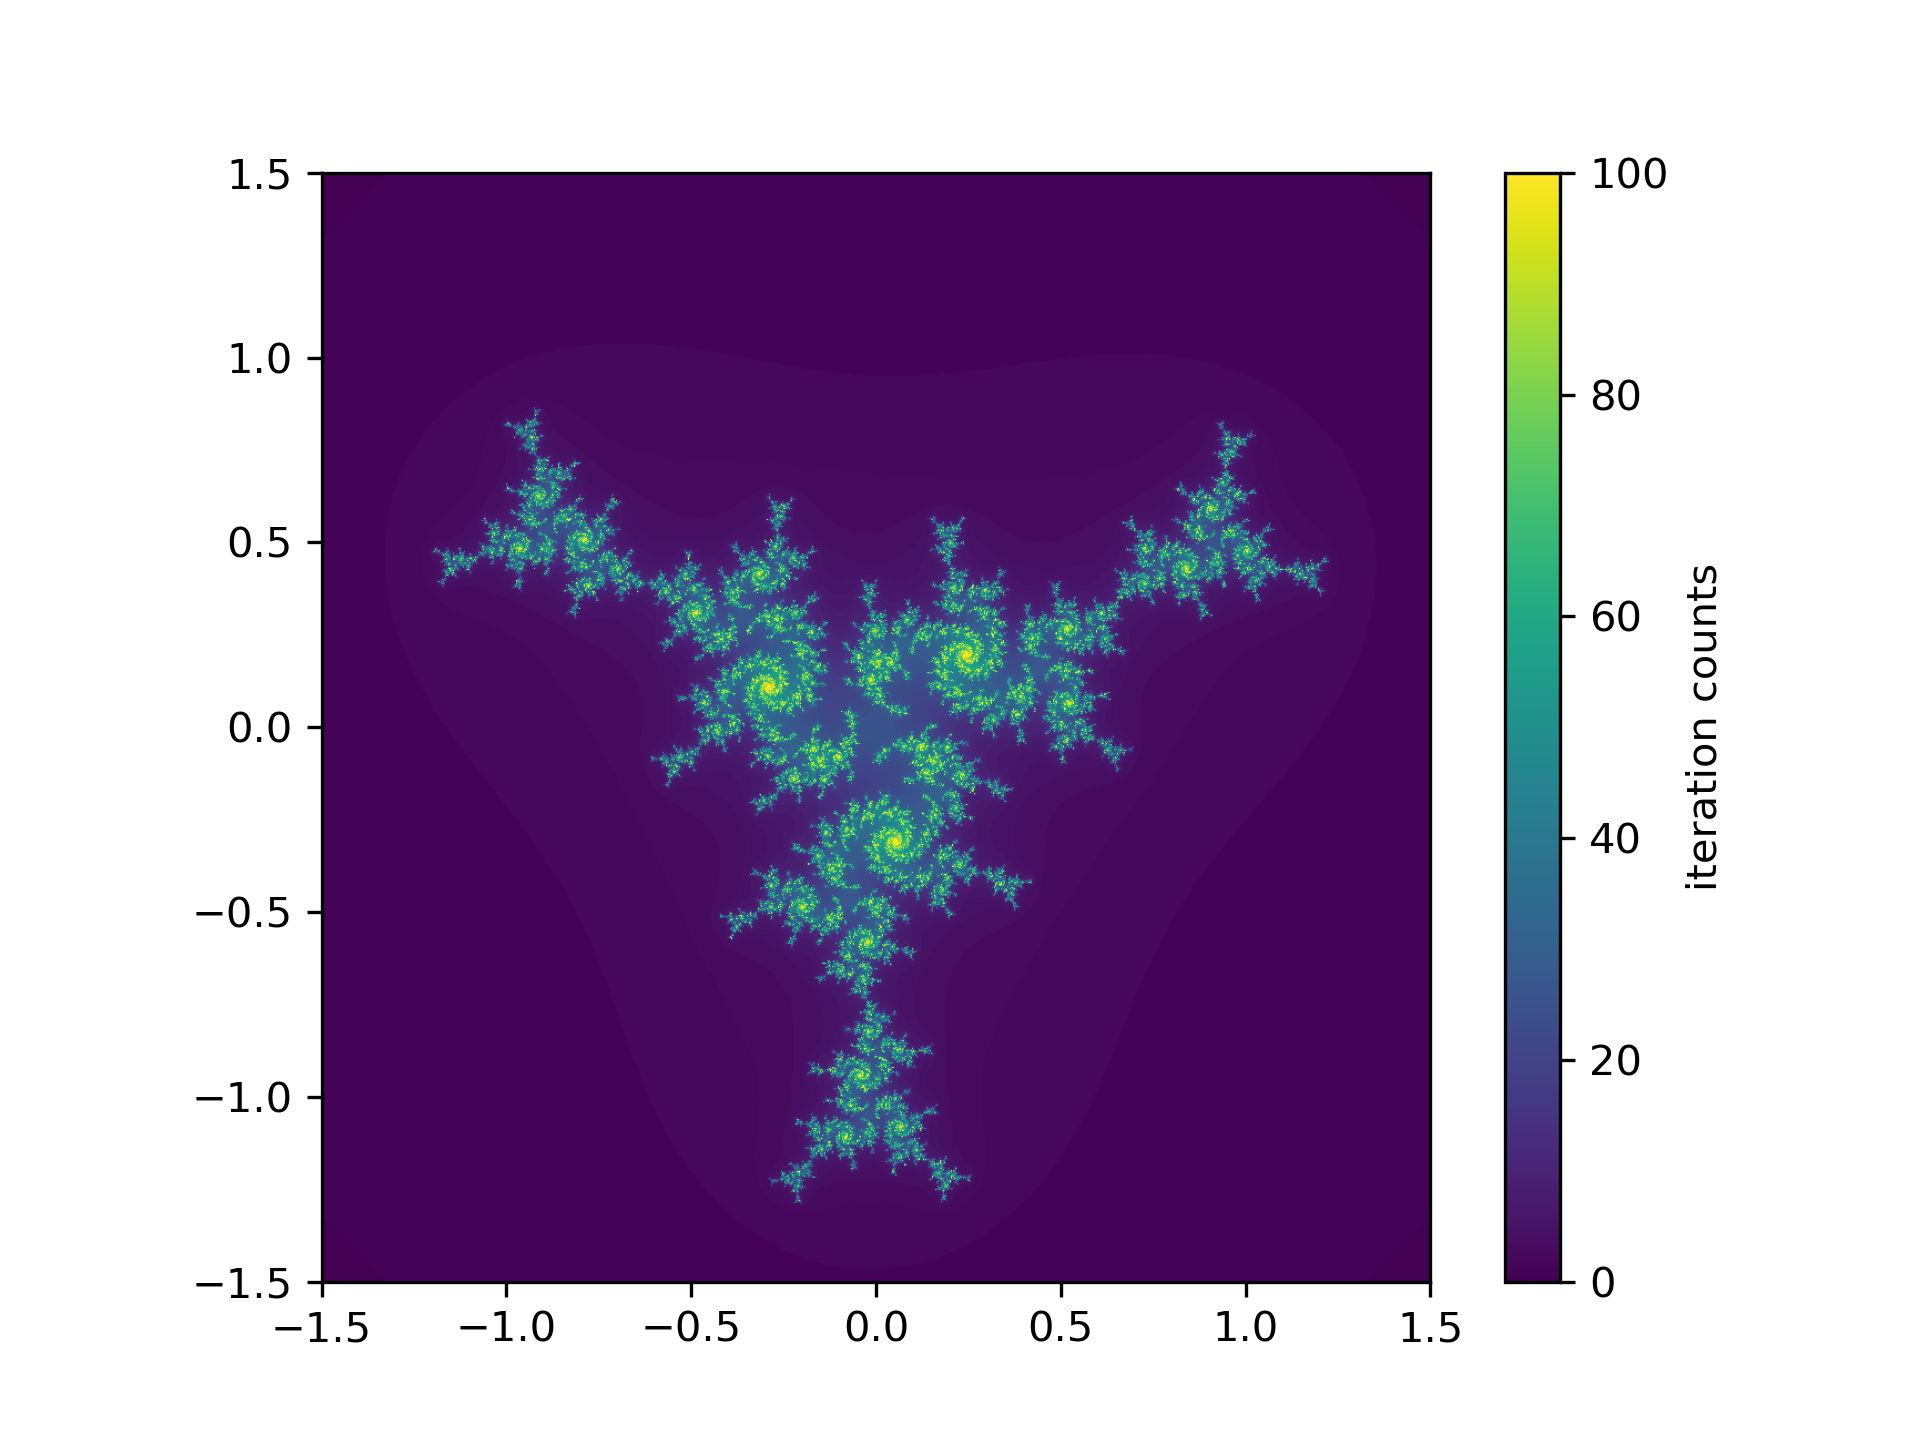
\includegraphics[width=.45\textwidth]{../png/300dpi/julia_f1_N100.png}
	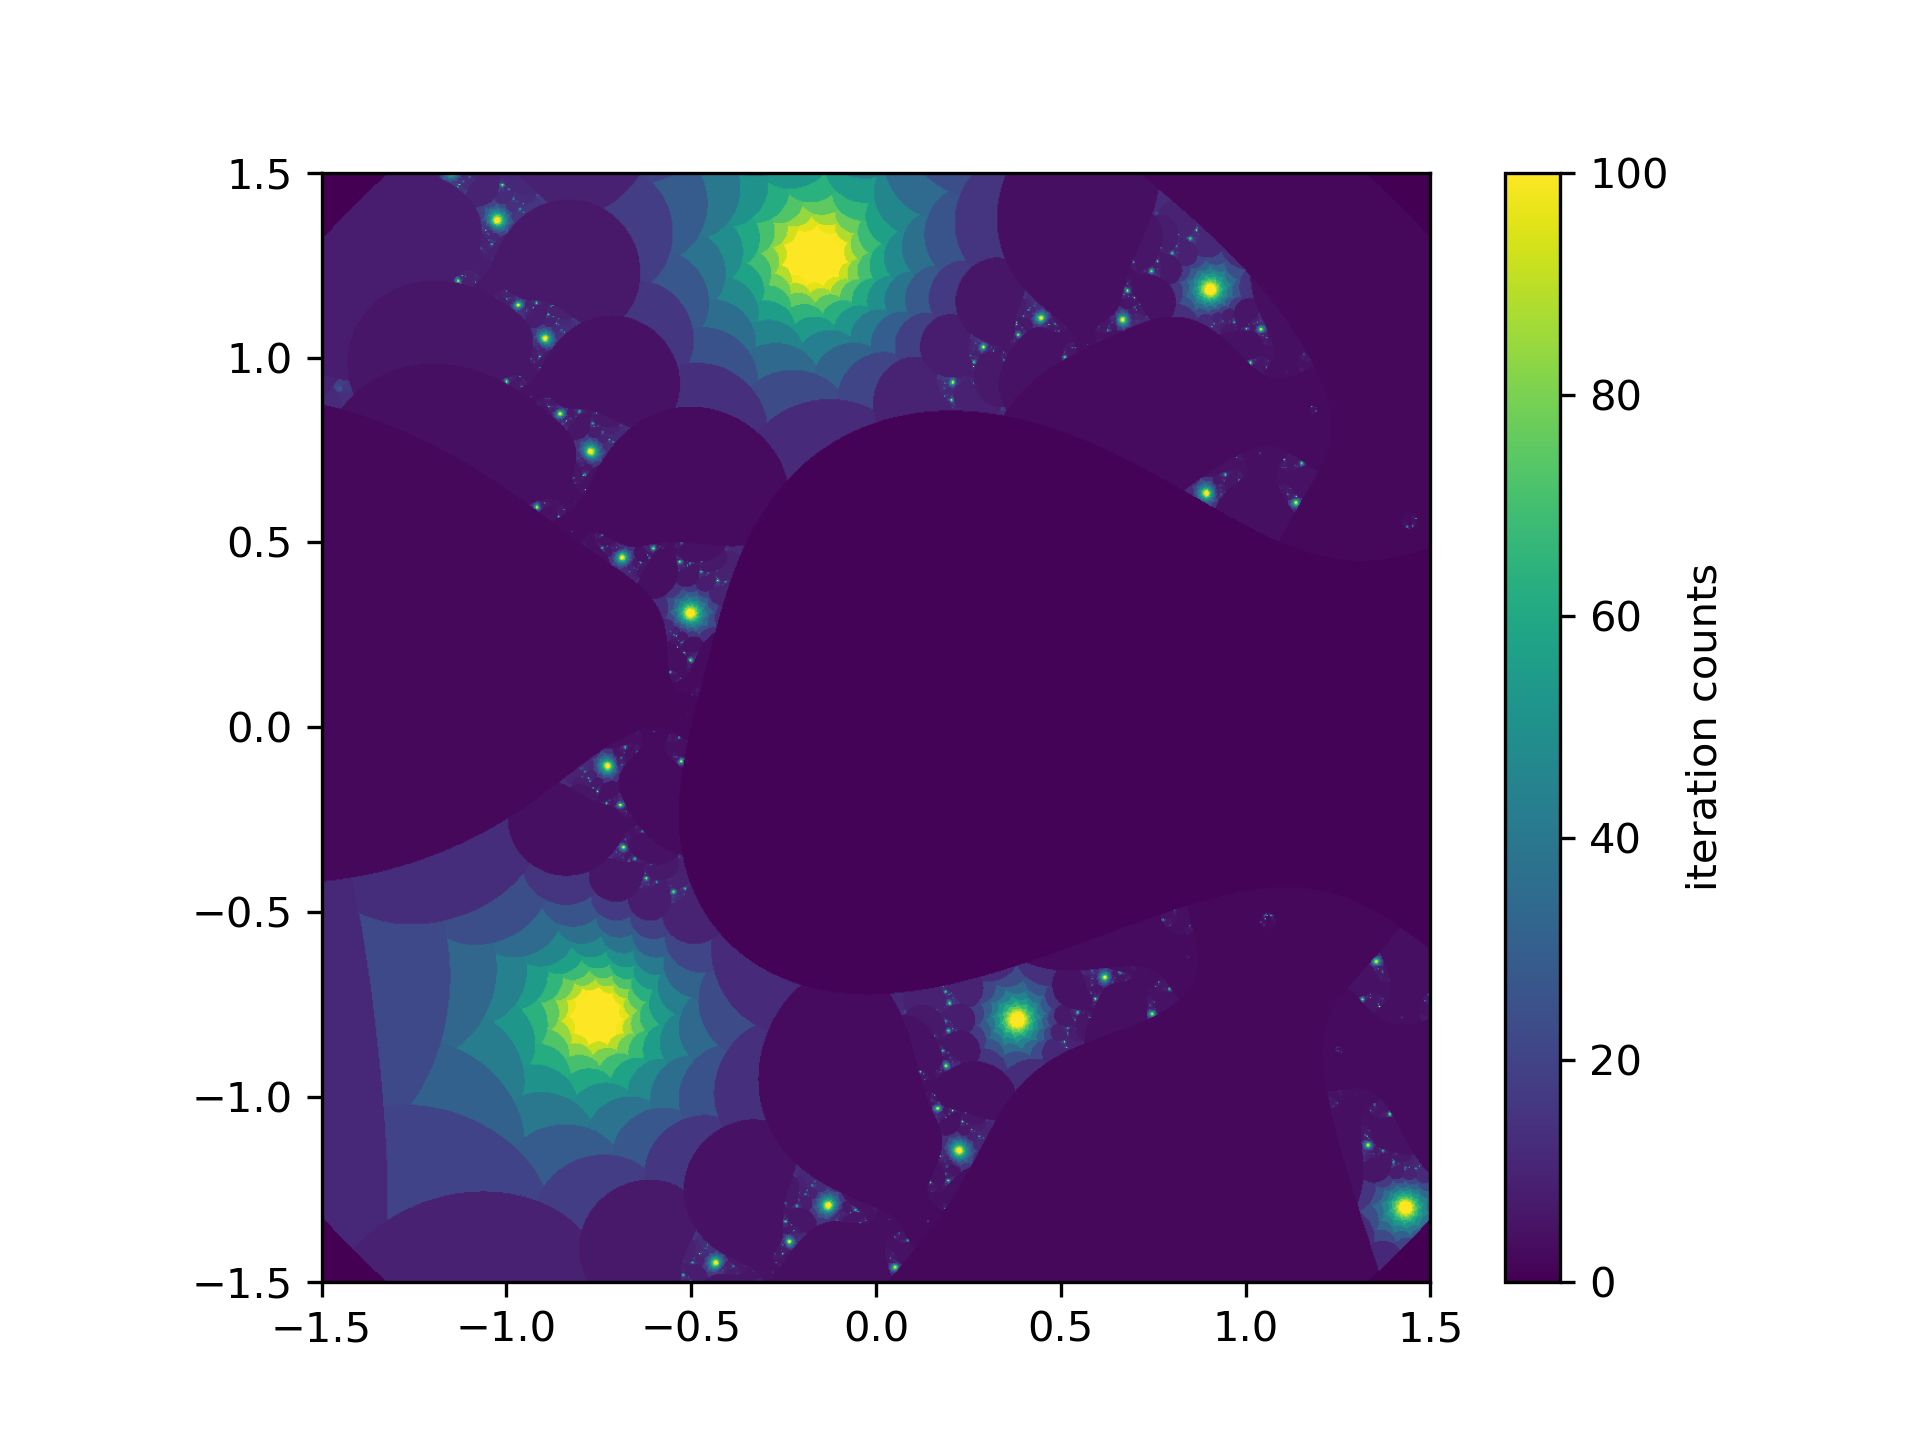
\includegraphics[width=.45\textwidth]{../png/300dpi/julia_f2_N100.png}
	\caption{$N=100,f(z)=f_1(z),f_2(z)$}
\end{figure}
\end{frame}

\begin{frame}{拓展:Julia集和Mandelbrot集之间的关系}
\section{拓展:Julia集和Mandelbrot集之间的关系}
\begin{itemize}
\item 实际上Julia集和Mandelbrot集就是同一函数$f(z)$对不同参数的递归过程。
\item Julia集是固定复常数$c$,取遍复数$z$进行递归。
\item Mandelbrot集则是固定递归初值$z_0$取遍复数$c$进行递归。
\item 更深入的来看,Mandelbrot集就是对Julia集的一个概括,这是因为在Mandelbrot集中所选取的$c$值对应到Julia集时,这个Julia集是连通的,反之亦然。
\end{itemize}
\end{frame}

\begin{frame}{总结与思考}
\section{总结与思考}
\begin{itemize}
\item 通过以上简单的分析与探索,我对Julia集的性质与特征有了更深入的了解,并且通过Python语言仿照编写了程序对分析和探索的过程进行了可视化,使得这一过程更为清晰自然。
\item 同时还对Mandelbrot集与Julia集的关系进行了浅显的分析与观察,而这一联系方法想必能够适用于其他的$f(z)$,这将帮助我们寻找不同$f(z)$下更能凸显图像性质的$c$值。
\end{itemize}
\end{frame}

\end{document}
